\documentclass[12pt,a4paper]{report}
\usepackage[left=3.00cm, right=2.00cm, top=2.00cm, bottom=2.00cm]{geometry}
\usepackage{vntex}
\usepackage{amsmath}
\usepackage{amssymb}
\usepackage{graphicx}
\author{LHD}
\newcommand{\nocontentsline}[3]{}
\newcommand{\tocless}[2]{\bgroup\let\addcontentsline=\nocontentsline#1{#2}\egroup}
\author{LHD}
\usepackage{tikz}
\usetikzlibrary{calc}
\title{Đề cương Ver 1}

\begin{document}
\begin{titlepage}
	\begin{tikzpicture}[remember picture,overlay,inner sep=0,outer sep=0]
		\draw[blue!70!black,line width=4pt] ([xshift=-1.5cm,yshift=-2cm]current page.north east) coordinate (A)--([xshift=1.5cm,yshift=-2cm]current page.north west) coordinate(B)--([xshift=1.5cm,yshift=2cm]current page.south west) coordinate (C)--([xshift=-1.5cm,yshift=2cm]current page.south east) coordinate(D)--cycle;
		
		\draw ([yshift=0.5cm,xshift=-0.5cm]A)-- ([yshift=0.5cm,xshift=0.5cm]B)--
		([yshift=-0.5cm,xshift=0.5cm]B) --([yshift=-0.5cm,xshift=-0.5cm]B)--([yshift=0.5cm,xshift=-0.5cm]C)--([yshift=0.5cm,xshift=0.5cm]C)--([yshift=-0.5cm,xshift=0.5cm]C)-- ([yshift=-0.5cm,xshift=-0.5cm]D)--([yshift=0.5cm,xshift=-0.5cm]D)--([yshift=0.5cm,xshift=0.5cm]D)--([yshift=-0.5cm,xshift=0.5cm]A)--([yshift=-0.5cm,xshift=-0.5cm]A)--([yshift=0.5cm,xshift=-0.5cm]A);
		
		
		\draw ([yshift=-0.3cm,xshift=0.3cm]A)-- ([yshift=-0.3cm,xshift=-0.3cm]B)--
		([yshift=0.3cm,xshift=-0.3cm]B) --([yshift=0.3cm,xshift=0.3cm]B)--([yshift=-0.3cm,xshift=0.3cm]C)--([yshift=-0.3cm,xshift=-0.3cm]C)--([yshift=0.3cm,xshift=-0.3cm]C)-- ([yshift=0.3cm,xshift=0.3cm]D)--([yshift=-0.3cm,xshift=0.3cm]D)--([yshift=-0.3cm,xshift=-0.3cm]D)--([yshift=0.3cm,xshift=-0.3cm]A)--([yshift=0.3cm,xshift=0.3cm]A)--([yshift=-0.3cm,xshift=0.3cm]A);
		
	\end{tikzpicture}
	\begin{center}
		BAN CƠ YẾU CHÍNH PHỦ\\
		\textbf{HỌC VIỆN KỸ THUẬT MẬT MÃ}
	\end{center}
	\begin{figure}[h]
		\centering
		\includegraphics[width=0.25\linewidth]{"Pics/Logo HV"}
		\label{fig:logo-hv}
	\end{figure}
	
	\begin{center}
		{\Huge ĐỀ CƯƠNG\\}
		{\large CHUYÊN ĐỀ AN TOÀN HỆ THỐNG THÔNG TIN\\}
		\textbf{Nghiên cứu giải pháp đảm bảo an toàn cho Microservices trên Kubernetes}
	\end{center}
	\bigskip
	\begin{flushright}
		\large{Ngành: An toàn thông tin}
	\end{flushright}
	\vspace{30mm}
	\begin{flushleft}
		\textit{Sinh viên thực hiện:}\\
		\textbf{Phương Văn Sơn}\\
		Mã sinh viên: AT160258\\
		\textbf{Lê Huy Dũng}\\
		Mã sinh viên: AT160211
		\bigskip\\
		\textit{Người hướng dẫn:}\\
		\textbf{TS. Nguyễn Mạnh Thắng}\\
		Khoa An toàn thông tin - Học viện Kỹ thuật mật mã
	\end{flushleft}
	\vfill
	\begin{center}
		Hà Nội, 2022
	\end{center}
	
\end{titlepage}

	\tableofcontents
	
	\chapter*{\centering Lời cảm ơn}
	\addcontentsline{toc}{chapter}{Lời cảm ơn}
	\hspace{1cm}Nhóm chúng em xin chân thành cảm ơn các thầy cô trường Học viện Kỹ thuật Mật mã nói chung, quý thầy cô của khoa An toàn thông tin nói riêng đã tận tình dạy bảo, truyền đạt kiến thức cho chúng em trong suốt quá trình học.\newline
	
	\hspace{1cm} Kính gửi đến Thầy Nguyễn Mạnh Thắng lời cảm ơn chân thành và sâu sắc nhất, cảm ơn thầy đã tận tình theo sát, chỉ bảo và hướng dẫn cho nhóm em trong quá trình thực hiện đề tài này. Thầy không chỉ hướng dẫn chúng em những kiến thức chuyên ngành, mà còn giúp chúng em học thêm những kĩ năng mềm, tinh thần học hỏi, thái độ khi làm việc nhóm.\\
	
	\hspace{1cm}Trong quá trình tìm hiểu nhóm chúng em xin cảm ơn các bạn sinh viên đã góp ý, giúp đỡ và hỗ trợ nhóm em rất nhiều trong quá trình tìm hiểu và làm đề tài.\\
	
	\hspace{1cm}Do kiến thức còn nhiều hạn chế nên không thể tránh khỏi những thiếu sót trong quá trình làm đề tài.Chúng em rất mong nhận được sự đóng góp ý kiến của quý thầy cô để đề tài của chúng em đạt được kết quả tốt hơn.\\
	\bigskip \\
	\textbf{Chúng em xin chân thành cảm ơn!}
	\chapter*{\centering Lời mở đầu}
	\addcontentsline{toc}{chapter}{Lời mở đầu}
	\hspace{1cm}{Nhiều năm trước, hầu hết các ứng dụng phần mềm đều được xây dựng với kiến trúc monolith hay còn gọi là kiến trúc 1 khối là mẫu thiết kế được dùng nhiều nhất trong giới lập trình web hiện nay bởi tính đơn giản của nó khi phát triển và khi triển khai. Các ứng dụng này chạy dưới dạng một tiến trình đơn lẻ hoặc số lượng nhỏ các tiến trình trên một số ít máy chủ. Chúng có khả năng cập nhật và nâng cấp chậm và yêu cầu nâng cấp thường xuyên. Trong trường hợp có sự cố như lỗi phần cứng hệ thống phần mềm này sẽ phải được di chuyển một cách thủ công sang các máy chủ còn hoạt động tốt.\\}
	
	{\hspace{0.3cm}Ngày nay các ứng dụng được xây dựng với kiến trúc lớn và phức tạp đang dần được chia thành các thành phần nhỏ hơn, có khả năng hoạt đông độc lập được gọi là microservices. Vì các Microservices tách biệt với nhau nên chúng có thể được phát triển, triển khai hay cập nhật và mở rộng quy mô một cách riêng lẻ. Nhờ khả năng này cho phép ta thay đổi các thành phần nhanh chóng và thường xuyên khi cần thiết để theo kịp với các yêu cầu thay đổi nhanh chóng thời nay.\\}
	
	\hspace{0.3cm}Nhưng với số lượng lớn các thành phần cũng như cơ sở dữ liệu việc cấu hình, quản lý và giữ hệ thống hoạt động trơn tru ngày càng trở nên khó khăn đặc biệt trong việc tối ưu hiệu quả sử dụng tài nguyên. Kubernetes ra đời ể đáp ứng nhu cầu tự động hoá như lập lịch tự động, cấu hình tự động hay giám sát và xử lý lỗi.\\
	
	\hspace{0.3cm}Kubernetes cung cấp cho các nhà phát triển khả năng triển khai các ứng dụng một cách thường xuyên mà không cần thông qua nhóm vận hành. Không chỉ dừng lại ở đó Kuberbetes cũng giúp nhóm vận hành tự động theo dõi và khắc phục sự cố. \\
	
	\hspace{0.3cm}Đi cùng với sự phát triển lớn mạnh của kiến trúc Microservices cũng như Kubernetes đó là nhu cầu về việc đảm bảo tính an toàn cho các hệ thống này. Trong bài báo cáo này chúng em sẽ giới thiệu về giải pháp đảm bảo an toàn cho Microservices bằng Istio Service Mesh
	
	\chapter{Giới thiệu về công nghệ Container và kiến trúc Microservices}
		\section{Giới thiệu về công nghệ Container}
		\smallskip
		{\hspace{1cm}Xây dựng phần mềm theo xu hướng Cloud Native đang phát triển rất nhanh. Trong đó, công nghệ container đóng 1 vai trò rất quan trọng để theo đuổi cách triển khai này.}
			
		{\hspace{0,3cm}Công nghệ container, hay gọi đơn giản là container, là một phương pháp đóng gói ứng dụng để ứng dụng có thể chạy với các phụ thuộc của mình (gồm source code và library, runtime, framework…) một cách độc lập, tách biệt với các chương trình khác. Các nhà cung cấp dịch vụ đám mây lớn hiện nay đã cung cấp các dịch vụ dành cho việc quản lý container để hỗ trợ việc xây dựng ứng dụng sử dụng công nghệ container.}
		\subsection{Hiểu về công nghệ Container}
		\hspace{1cm}Container được đặt tên theo thuật ngữ container của ngành vận tải biển vì có cùng chung ý tưởng với nhau. Thay vì chỉ vận chuyển từng sản phẩm, hàng hóa được đặt vào các thùng hàng bằng thép, được thiết kế theo các tiêu chuẩn phù hợp về kích thước và trọng tải để có thể cẩu lên bến tàu và lắp vào con tàu. Như vậy, bằng cách tiêu chuẩn hóa quy trình và nhóm các thành phần liên quan lại với nhau, từng container sẽ được chuyển đi riêng lẻ và sẽ tốn ít chi phí hơn để làm theo cách này.
		
		\hspace{0,3cm}Trong công nghệ, tình huống cũng khá tương tự. Một chương trình chạy hoàn hảo trên một máy, nhưng khi chuyển sang máy khác thì lại không hoạt động được. Điều này có thể xảy ra khi di chuyển phần mềm từ PC của developer sang test server hoặc từ server vật lý sang cloud server. Các vấn đề phát sinh khi di chuyển phần mềm là do sự khác biệt giữa các môi trường máy tính, chẳng hạn như OS, thư viện SSL, storage, bảo mật và cấu trúc mạng trên các máy khác nhau sẽ khác nhau..
		
		\hspace{0,3cm}Container giải quyết vấn đề trên bằng cách tạo ra một môi trường bị cô lập (isolated) chứa mọi thứ mà phần mềm cần để có thể chạy được mà không bị các yếu tố liên quan đến môi trường hệ thống làm ảnh hưởng tới cũng như không làm ảnh hưởng tới các phần còn lại của hệ thống.
		
		\hspace{0,3cm}Giống như việc toàn bộ 1 container sẽ được nhấc lên tàu hoặc xe tải để vận chuyển, công nghệ container cũng như vậy. Container không chỉ chứa phần mềm mà còn chứa các phần phụ thuộc bao gồm các library, binary và file cấu hình cùng với nhau và chúng được di chuyển như một bộ phận, để tránh sự không tương thích và sự cố. Các container giúp việc triển khai phần mềm lên máy chủ thuận lợi hơn.
		
		\hspace{0,3cm}Như vậy, những container có tác dụng giúp cho một ứng dụng có thể vận hành một cách nhất quán và đáng tin cậy. Bất kể là môi trường hệ điều hành hay cơ sở hạ tầng nào. Các container thực hiện điều này bằng cách đóng gói mọi thứ mà một dịch vụ cần để có thể chạy được (những thứ như code, runtime, các tool, thư viện và cài đặt), tạo ra một package linh động, độc lập, có khả năng thực thi được.
		\subsection{Container và Máy ảo}
		\hspace{1cm}Trước khi các container dần được ưa chuộng, máy ảo VM là một phương pháp sử dụng phổ biến. Ở phương pháp này, một máy chủ vật lý có thể được sử dụng cho nhiều ứng dụng thông qua công nghệ ảo hóa, còn được gọi là virtual machine, trong đó mỗi máy ảo chứa toàn bộ hệ điều hành, cũng như các ứng dụng cần thiết để chạy.
		\subsubsection{Về cấu trúc}
		\hspace{1cm}VM, hay Virtual Machine/máy ảo là một phiên bản tóm tắt của máy tính, từ hệ điều hành cho đến bộ nhớ và lưu trữ. Image dùng để tạo một VM có thể tương tự hệ điều hành để cài đặt ứng dụng lên hoặc có sẵn tất cả các ứng dụng bạn cần, như web server và database, thậm chí cả chính ứng dụng của bạn. Mỗi VM sẽ hoạt động độc lập hoàn toàn với máy chủ mà VM chạy trên đó, cũng như độc lập với bất kỳ VM nào khác trên máy chủ đó.

		\hspace{0,3cm}Trong khi đó, container sẽ chạy một phần của máy hiện có, chia sẻ kernel của máy chủ đó với bất kỳ container nào khác đang chạy trên hệ thống. Chỉ chứa vừa đủ hệ điều hành và bất kỳ thư viện hỗ trợ nào cần thiết để chạy code. Container được xây dựng từ những image bao gồm mọi thứ nó cần - và không có gì khác (trong TH lý tưởng nhất).
		\subsubsection{Nhu cầu tài nguyên}
		\hspace{1cm}Do cấu trúc khác nhau nên nhu cầu để chạy VM và container có thể khác nhau đáng kể. Bởi vì về cơ bản VM tương đương với toàn bộ một máy tính, nên đương nhiên sẽ cần nhiều tài nguyên hơn là một container, trong khi container chỉ cần đến một phần nhỏ nhất của hệ điều hành. Tóm lại, việc mở rộng các container sẽ ít tốn tài nguyên, thời gian, công sức hơn và có thể “xếp” nhiều container hơn trên một máy chủ duy nhất.
		
		\hspace{0,3cm}Tuy nhiên, cần hết sức lưu ý là vì nhiều dịch vụ có thể “chia sẻ” tài nguyên của một máy ảo duy nhất, có thể có những trường hợp phức tạp trong đó cần thiết phải mở rộng nhiều container để thay thế một máy ảo duy nhất. Điều này dẫn đến việc kiểm soát tài nguyên không còn nhiều ý nghĩa. Ví dụ: nếu bạn tách một máy ảo đơn lẻ thành 50 dịch vụ khác nhau, thì đó là 50 bản sao một phần của hệ điều hành so với một bản sao đầy đủ. Vì vậy, điều quan trọng là cần hiểu chính xác để lựa chọn đúng.
		
		\hspace{0,3cm}Vậy Container và máy ảo thì đều là những “package”. Mỗi container là một package bao gồm ứng dụng của bạn và mọi thứ nó cần để có thể chạy, ngoại trừ hệ điều hành. Máy ảo là một package ứng dụng và mọi thứ nó cần để chạy, bao gồm cả hệ điều hành của nó.
		
		\hspace{0,3cm}Bạn có thể chạy nhiều container trên một hệ điều hành. Và bạn có thể chạy nhiều máy ảo trên cùng một máy chủ vật lý. Bạn thậm chí có thể chạy container trên máy ảo.
		
		\hspace{0,3cm}Một lợi thế quan trọng của container so với máy ảo đó là chúng không bao gồm hệ điều hành, container cần ít tài nguyên hệ thống và ít chi phí hơn. Chúng cũng có xu hướng khởi động / tắt nhanh hơn và tính di động cao trong nhiều môi trường khác nhau. Nhưng chúng vẫn sử dụng công suất cơ sở hạ tầng khi không sử dụng, điều này có thể làm tăng chi phí không cần thiết.
		\subsection{Đặc điểm kỹ thuật của Container}
		\hspace{1cm}Mô hình kiến trúc của container bao gồm các thành phần chính là Server (máy chủ vật lý hoặc máy ảo), host OS (hệ điều hành cài đặt trên server) và các container.
		
		\hspace{0,3cm}Mỗi một ứng dụng (App A và App B) sẽ có những sự phụ thuộc riêng của nó bao gồm cả về phần mềm (các dịch vụ hay thư viện) lẫn cả về phần cứng (CPU, bộ nhớ, lưu trữ).
		
		\hspace{0,3cm}Các ứng dụng này sẽ được Container Engine, một công cụ ảo hóa tinh gọn, được cài đặt trên host OS, nó sẽ cô lập sự phụ thuộc của các ứng dụng khác nhau bằng cách đóng gói chúng thành các container. Các tiến trình (process) trong một container bị cô lập với các tiến trình của các container khác trong cùng hệ thống tuy nhiên tất cả các container này đều chia sẻ kernel của host OS (dùng chung host OS).
		
		\hspace{0,3cm}Với mô hình trên, sự phụ thuộc của ứng dụng vào tầng OS cũng như cơ sở hạ tầng được loại bỏ giúp việc triển khai phương pháp “deploy anywhere” (triển khai ở bất kỳ nơi đâu) của container được hiệu quả hơn. Thêm vào đó, do chia sẻ host OS nên container có thể được tạo gần như một cách tức thì, giúp việc scale-up và scale-down theo nhu cầu được thực hiện một cách nhanh chóng.
		\subsection{Ứng dụng của Container trong thực tế}
		\hspace{1cm}Các container đại diện cho tương lai của máy tính cùng với các công nghệ như DevOps, cloud native, AI, machine learning. Các trường hợp sử dụng phổ biến bao gồm:
		\begin{itemize}
		\item Hiện đại hóa các ứng dụng hiện có trên đám mây
		\item Tạo các ứng dụng mới tối đa hóa lợi ích của container
		\item Cô lập, triển khai, mở rộng quy mô và hỗ trợ microservices và các ứng dụng phân tán
		\item Tăng cường hiệu quả DevOps, hiệu quả thông qua việc build/test/triển khai được sắp xếp một cách hợp lý
		\item Cung cấp cho nhà phát triển một môi trường sản xuất nhất quán, tách biệt khỏi các ứng dụng và quy trình khác
		\item Đơn giản hóa và tăng tốc các chức năng có tính lặp đi lặp lại\\
		\end{itemize}
		
		\hspace{0,3cm}Tạo điều kiện thuận lợi cho các môi trường máy tính kết hợp với multi-cloud, vì các container có thể chạy nhất quán ở bất kỳ đâu.
		\subsection{Về Containerization}
		\hspace{1cm}Containerization là hành động tạo một container, bao gồm việc chỉ lấy ra ứng dụng hay dịch vụ mà bạn cần chạy, cùng với các cấu hình và những phần phụ thuộc của nó, đồng thời rút nó ra khỏi hệ điều hành và cơ sở hạ tầng bên dưới. Sau đó, cho ra kết quả là container image có thể chạy trên bất kỳ nền tảng container nào.
		
		\hspace{0,3cm}Nhiều container có thể được chạy trên cùng một máy chủ và chia sẻ cùng một hệ điều hành với các container khác, mỗi container chạy các quy trình biệt lập trong không gian được bảo mật riêng của nó. Bởi vì các container chia sẻ base OS (hệ điều hành), do vậy kết quả là có thể chạy mỗi container bằng cách sử dụng một lượng tài nguyên rất ít, ít hơn đáng kể so với việc sử dụng số lượng máy ảo (VM) riêng biệt.
		\subsubsection{Những lợi ích của Container}
		\subsubsection{Tốn rất ít dung lượng}
		\hspace{1cm}Các container chia sẻ kernel của máy chủ lưu trữ, chúng chỉ chứa các thành phần thực sự cần thiết với hệ điều hành và thư viện. Đồng thời các container thường cũng chỉ giới hạn ở một chức năng duy nhất, nên có kích thước rất nhỏ. Nhờ vậy, việc xây dựng, triển khai cực kỳ nhanh chóng.
		
		\hspace{0,3cm}Bởi vì chúng được tách biệt khỏi lớp OS nên việc container chạy hiệu quả và nhẹ về tài nguyên hơn so với máy ảo cũng là điều dễ hiểu.
		\subsubsection{Các Container có tính linh hoạt}
		\hspace{1cm}Vì container bao gồm có tất cả các cấu hình cần thiết và các thành phần phụ thuộc, do vậy bạn có thể viết một lần và di chuyển giữa các môi trường. Có một câu thần chú nổi tiếng đó là “Build once, run everywhere”.\\
		\begin{itemize}
			\item \textbf{Triển khai nhanh:}
			\subitem Do kích thước nhỏ, các container có thể chỉ cần vài giây để khởi động, thậm chí là ít hơn, nên rất thích hợp cho các ứng dụng cần được đẩy lên và xuống liên tục, chẳng hạn như các ứng dụng “serverless”.
			\item \textbf{\textbf{CI/CD:}}
			\subitem 
			CI là tên viết tắt của Continuous Integration, theo nghĩa tiếng Việt là tích hợp liên tục. Quá trình hoạt động cho phép các thành viên trong một team liên tục lưu trữ những mã mới vào một kho nhất định. Nhờ vào số lượng dữ liệu này, CI sẽ tự động chạy test và kiểm tra độ chính xác. Cùng lúc đó cũng hỗ trợ phát triển phần mềm một cách nhanh chóng hơn bằng việc báo lỗi sai và đưa ra gợi ý giải quyết.
			
			\hspace{0,8cm}CD là tên viết tắt của Continuous Delivery, nghĩa là quá trình chuyển giao liên tục. Về cơ bản, CD cũng sở hữu những kỹ năng của CI, tuy nhiên sẽ phức tạp và nâng cao hơn một chút.
			
			\hspace{0,8cm}Trong khi CI chỉ chạy và kiểm tra những code đã có sẵn, CD thậm chí còn tự sửa code đã được build và test nếu phát hiện lỗi sai. Ngoài ra, nó cũng tự động thay đổi môi trường testing hoặc staging để nâng cao chất lượng kiểm tra.
			
			\hspace{0,8cm}Chính vì các container được thiết kế để có thể start và restart thường xuyên, nhờ vậy mà dễ dàng tiếp nhận các thay đổi tạo điều kiện vô cùng phù hơp để triển khai CI/CD.
			\item \textbf{Khả năng mở rộng:}
			\subitem Do kích thước nhỏ của chúng, các container có thể dễ dàng lấy ra, mở rộng quy mô trong quá trình vận hành, tắt đi khi không sử dụng và nhanh chóng khởi động lại khi cần thiết.
			\item \textbf{Tiết kiệm chi phí:}
			\subitem Thông qua việc giảm lượng nhu cầu về tài nguyên và mở rộng quy mô một cách thông minh, các container cung cấp một giải pháp linh hoạt, nhanh chóng và tiết kiệm chi phí.
		\end{itemize}
		\subsubsection{Khả năng chịu lỗi cao}
		\hspace{1cm}Các nhóm phát triển phần mềm sử dụng bộ chứa để xây dựng các ứng dụng có khả năng chịu lỗi cao. Họ sử dụng nhiều bộ chứa để chạy vi dịch vụ trên đám mây. Bởi vì các vi dịch vụ trong bộ chứa hoạt động trong không gian người dùng riêng biệt, một bộ chứa bị lỗi riêng lẻ sẽ không ảnh hưởng đến các bộ chứa khác. Điều này làm tăng khả năng phục hồi và tính khả dụng của ứng dụng.
		\subsubsection{Quản lý ít cơ sở hạ tầng hơn}
		\hspace{1cm}Container buộc bạn phải nắm bắt được những gì mà bạn thực sự cần qua đó mang lại trải nghiệm tốt nhất cho khách hàng của bạn. Điều này giúp quản lý cơ sở hạ tầng tốt hơn vì đơn giản là có ít cơ sở hạ tầng hơn để quản lý.
		\subsubsection{Container tạo ra khả năng tập trung}
		\hspace{1cm}Các teams IT sẽ dành ít thời gian hơn cho các hệ điều hành và phần cứng, điều đó cho phép họ tập trung hơn vào các dự án quan trọng của doanh nghiệp.
		\subsubsection{Thúc đẩy sự phát triển}
		\hspace{1cm}Container cung cấp một môi trường ổn định, dễ dàng dự đoán được, nơi CPU/memory được tối ưu hóa và code thì được trừu tượng hóa từ cơ sở hạ tầng để có tính khả chuyển.
		\subsubsection{Tạo điều kiện cho những kiến trúc hiện đại}
		\hspace{1cm}Sử dụng container, các nhà phát triển có thể chia các ứng dụng thành các microservices, điều này có thể tăng tốc độ phát triển và khi được triển khai thì được mở rộng một cách riêng biệt.
		\subsection{Những thách thức trong việc sử dụng Container}
		\subsubsection{Container còn tương đối mới}
		\hspace{1cm}Kubernetes được phát hành lần đầu tiền vào năm 2014 và nhanh chóng được thị trường đón nhận. Việc trở thành một “hot tech” có thể gây khó khăn trong việc tìm kiếm những người có kinh nghiệm và biết cách làm việc với nhiều môi trường container.
		\subsubsection{Không phải dịch vụ nào cũng được hỗ trợ Container hóa}
		\hspace{1cm}Nếu ứng dụng của bạn đưa vào các dịch vụ không hỗ trợ container. Bạn có thể cần phải đầu tư nhiều để chuyển đổi nó thành một giải pháp container.
		\subsubsection{Container yêu cầu nhiều thay đổi về quy trình và kỹ năng}
		\hspace{1cm}Container có thể đẩy nhanh quá trình chuyển đổi của bạn sang kiểu phát triển agile hay eficient, nhưng điều này cũng đồng nghĩa với với việc tạo ra một thay đổi lớn đối với các quy trình hiện có như quy trình phát triển, triển khai, review và giám sát. Dẫn đến việc các team mà tổ chức hiện có cần phải được điều chỉnh và đào tạo lại.
		\begin{itemize}
			\item \textbf{Có thể yêu cầu kết nối mạng phức tạp: }
			\subitem Thường thường các chức năng sẽ được chia thành nhiều container và cần phải giao tiếp với nhau. Việc số lượng rất nhiều các container phải giao tiếp với nhau có thể phức tạp. Một số hệ thống điều phối như Kubernetes có các multi-container pods giúp việc trao đổi dễ dàng hơn một chút, nhưng được cho là vẫn phức tạp hơn so với sử dụng máy ảo. Thực tế thì mô hình mạng L3 trong Kubernetes đơn giản hơn nhiều so với mô hình L2 trong hạ tầng máy ảo OpenStack. Vì vậy, vấn đề nằm ở chỗ cần xác định được việc giao tiếp xảy ra giữa các chức năng hay giữa các máy ảo
			\item \textbf{Có thể cần thao tác nhiều hơn so với máy ảo:}
			\subitem Nếu sử dụng container, bạn sẽ phân tách ứng dụng thành các dịch vụ thành phần khác nhau, mặc dù việc này có ích lợi nhưng lại không cần thiết khi sử dụng VM.
			\item \textbf{Công nghệ đang phát triển với tốc độ chóng mặt:}
			\subitem Điều này không chỉ dành riêng cho container, nhưng về bản chất thì nhịp độ nhanh của công nghệ container có nghĩa là bạn cần mọi người (hoặc đối tác) có mặt để đưa ra quyết định đúng đắn, giảm rủi ro và đảm bảo việc triển khai không bị cản trở bởi tính trì trệ của công ty.
			\item \textbf{Container không phải là một viên đạn thần kỳ:}
			\subitem Đọc lướt qua một loạt các lợi ích thì trông có vẻ container là một thứ lý tưởng, nhưng hãy cẩn thận vì bất kỳ quá trình chuyển đổi nào cũng cần phải suy nghĩ nghiêm túc. Bạn phải biết mình đang làm gì, những gì sẽ mang lại hiệu quả và ngược lại. Hoặc tìm một ai có thể giúp bạn vượt trong sự chuyển đổi đó.
		\end{itemize}
		\section{Giới thiệu về kiến trúc Microservices}
		\hspace{1cm}Một vài năm trở lại đây, khái niệm kiến trúc Microservices hiện là chủ đề rất hot trong cộng động lập trình viên. Thật không khó để có thể tìm thấy một bài viết, một bản báo cáo hay một bài thuyết trình về chủ đề này. Vậy Microservices là gì? Ưu điểm và nhược điểm của kiến trúc Microservices ra sao?
		\subsection{Khái niệm Microservices}
		\hspace{1cm}Trong tiếng anh, micro có nghĩa là nhỏ, vi mô. Vậy Microservice, như tên của nó, đó chính là chia một khối phần mềm thành các service nhỏ hơn, có thể triển khai trên các server khác nhau. Mỗi service sẽ xử lý từng phần công việc và được kết nối với nhau thông qua các các giao thức khác nhau, như http, SOA, socket, Message queue (Active MQ, Kafka)... để truyền tải dữ liệu.
		
		\hspace{0,4cm}Trước khi Microservices xuất hiện, các ứng dụng thường phát triển theo mô hình Monolithic architecture (Kiến trúc một khối). Có nghĩa là tất cả các module (view, business, database) đều được gộp trong một project, một ứng dụng được phát triển theo mô hình kiến trúc một khối thường được phân chia làm nhiều module. Nhưng khi được đóng gói và cài đặt sẽ thành một khối (monolithic). Lợi ích của mô hình kiến trúc một khối đó là dễ dàng phát triển và triển khai. Nhưng bên cạnh đó nó cũng có nhiều hạn chế ví dụ như khó khăn trong việc bảo trì, tính linh hoạt và khả năng mở rộng kém, đặc biệt với những ứng dụng doanh nghiệp có quy mô lớn. Đó chính là lí do ra đời của kiến trúc Microservices.
		\subsection{Những đặc điểm của Microservices}
		\begin{description}
			\item[Decoupling:] Các service trong một hệ thống phần lớn được tách rời. Vì vậy, toàn bộ ứng dụng có thể dễ dàng được xây dựng, thay đổi và thu nhỏ.
			\item[Componentization:] Microservices được coi là các thành phần độc lập có thể dễ dàng thay thế và nâng cấp.
			\item[Business Capabilities:] Mỗi một thành phần trong kiến trúc microservice rất đơn giản và tập trung vào một nhiệm vụ duy nhất.
			\item[Autonomy:] Các lập trình viên hay các nhóm có thể làm việc độc lập với nhau trong quá trình phát triển.
			\item[Continous Delivery:] Cho phép phát hành phần mềm thường xuyên, liên tục.
			\item[Decentralized Governance:] Không có mẫu chuẩn hóa hoặc bất kỳ mẫu công nghệ nào. Được tự do lựa chọn các công cụ hữu ích tốt nhất để có thể giải quyết vấn đề.
			\item[Agility:] Microservice hỗ trợ phát triển theo mô hình Agile.
		\end{description}
		\subsection{Ưu điểm của Microservices}
		\hspace{0,4cm}Kiến trúc Microservices được sinh ra để khắc phục những hạn chế của kiến trúc một khối.
		\begin{itemize}
			\item Hoạt động độc lập, linh hoạt, có tính chuyên biệt cao: Do không bị ràng buộc bởi những yêu cầu chung, nên mỗi service nhỏ có thể tự do lựa chọn công nghệ, nền tảng phù hợp. Tất cả các service có thể được phát triển dễ dàng dựa trên chức năng cá nhân của từng service. Có thể chia nhỏ để phát triển độc lập.
			\item Nâng cao khả năng xử lý lỗi: Với mô hình này, một service bất kỳ nào gặp lỗi sẽ không gây ra ảnh hưởng đối với những bộ phận còn lại. Việc khắc phục lỗi trên quy mô hẹp cũng sẽ được tiến hành một cách dễ dàng, khi một service của ứng dụng không hoạt động, hệ thống vẫn tiếp tục hoạt động.
			\item Independent Deployment: Có thể được triển khai riêng lẻ trong bất kỳ ứng dụng nào.
			\item Mixed Technology Stack: Các ngôn ngữ và công nghệ khác nhau có thể được sử dụng để xây dựng các service khác nhau của cùng một ứng dụng.
			\item Thuận tiện trong nâng cấp, mở rộng: Tương tự như trường hợp xử lý lỗi, việc nâng cấp, bảo trì service hoàn toàn độc lập sẽ không làm gián đoạn quá trình vận hành của cả phần mềm. Nhờ vậy, những phiên bản mới có thể được cập nhật thường xuyên.
			\item Đơn giản hóa trong quản lý và kiểm thử: Với từng service nhỏ, các bước quản lý, tính toán và kiểm soát, xử lý lỗi sẽ trở nên đơn giản và nhanh chóng hơn so với cả phần mềm.
		\end{itemize}
		\hspace{0,4cm}Kiến trúc Microservices giúp đơn giản hóa hệ thống, chia nhỏ hệ thống ra làm nhiều service nhỏ lẽ dể dàng quản lý và triển khai từng phần so với kiến trúc nguyên khối. Phân tách rõ ràng giữa các service nhỏ. Cho phép việc mỗi service được phát triển độc lập. Cũng như cho phép lập trình viên có thể tự do chọn lựa technology stack cho mỗi service mình phát triển. mỗi service có thể được triển khai một cách độc lập (VD: Mỗi service có thể được đóng gói vào một docker container độc lập, giúp giảm tối đa thời gian deploy). Nó cũng cho phép mỗi service có thể được scale một cách độc lập với nhau. Việc scale có thể được thực hiện dễ dàng bằng cách tăng số instance cho mỗi service rồi phân tải bằng load balancer.
		\subsection{Các nhược điểm của kiến trúc Microservice}
		\hspace{1cm}Kiến trúc Microservices đang là một xu hướng, nhưng nó cũng có nhược điểm của nó.
		
		\hspace{0,4cm}Microservice khuyến khích làm nhỏ gọn các service, nhưng khi chia nhỏ sẽ dẫn đến những thứ vụn vặt, khó kiểm soát. Hơn nữa chính từ đặc tính phân tán khiến cho các lập trình viên phải lựa chọn cách thức giao tiếp phù hợp khi xử lí request giữa các service. Trong trường hợp dự án quá lớn, số lượng service nhiều, chia nhỏ rời rạc, thiếu tính liên kết. Cùng với cách thức liên kết thông tin giữa qua môi trường mạng, việc trao đổi giữa các service càng trở nên khó khăn. Đôi khi, các lỗi kết nối cũng có thể xảy ra khiến việc trao đổi này bị gián đoạn.
		
		\hspace{0,4cm}Việc liên tục di chuyển qua các database khác nhau sẽ khiến dữ liệu bị đảo lộn, không còn nguyên vẹn, thậm chí phải đối mặt với nguy cơ an ninh, bị đánh cắp.
		
		\hspace{0,4cm}Hơn nữa việc quản lí nhiều database, và transaction giữa các service trong một hệ thống phân tán cũng là một khó khăn không nhỏ. Hay khi thực hiện test một service, bạn cũng cần test các service có liên quan. Gây khó khăn trong quá trình mở rộng, phát triển. Khi phần mềm được phát triển với quy mô lớn hơn, số lượng service cũng trở nên nhiều hơn. Các lập trình viên không chỉ mất thời gian tính toán chính xác kích thước của từng service, mà còn gặp khó khăn khi sử dụng những công cụ hỗ trợ tự động mã nguồn mở bên ngoài khác.
		
		\hspace{0,4cm}Triển khai microservice cũng sẽ phức tạp hơn so với ứng dụng kiến trúc một khối, cần sự phối hợp giữa nhiều service, điều này không đơn giản như việc triển khai WAR trong một ứng dụng kiến trúc một khối.
		\subsection{Những yêu cầu bắt buộc khi phát triển phần mềm theo kiến trúc Microservice}
		\hspace{1cm}Để phát triển một phần mềm theo mô hình kiến trúc Microservice, lập trình viên cần đảm bảo một số yếu tố chính như sau:
		\begin{itemize}
			\item Xây dựng hệ cơ sở dữ liệu (database) độc lập.
			\item Xác định kích thước service phù hợp.
			\item Đề ra vai trò, chức năng cụ thể, riêng biệt cho từng service.
		\end{itemize}
		\hspace{0,4cm}Việc phát triển một phần mềm theo mô hình kiến trúc Microservice chưa bao giờ là điều đơn giản.
		\section{Giới thiệu về Kubernetes}
				{\hspace{0.6cm}Kubernetes là một nền tảng nguồn mở quản lý các ứng dụng được đóng gói và các service, giúp thuận lợi trong việc cấu hình và tự động hoá việc triển khai ứng dụng.\\}
				
				Tên gọi Kubernetes có nguồn gốc từ tiếng Hy Lạp, có ý nghĩa là người lái tàu hoặc hoa tiêu. Google mở mã nguồn Kubernetes từ năm 2014. Kubernetes xây dựng dựa trên một thập kỷ rưỡi kinh nghiệm mà Google có được với việc vận hành một khối lượng lớn workload trong thực tế, kết hợp với các ý tưởng và thực tiễn tốt nhất từ cộng đồng.\\
			\subsection{Kiến trúc của Kubernetes}
				\begin{figure}[h]
					\centering
					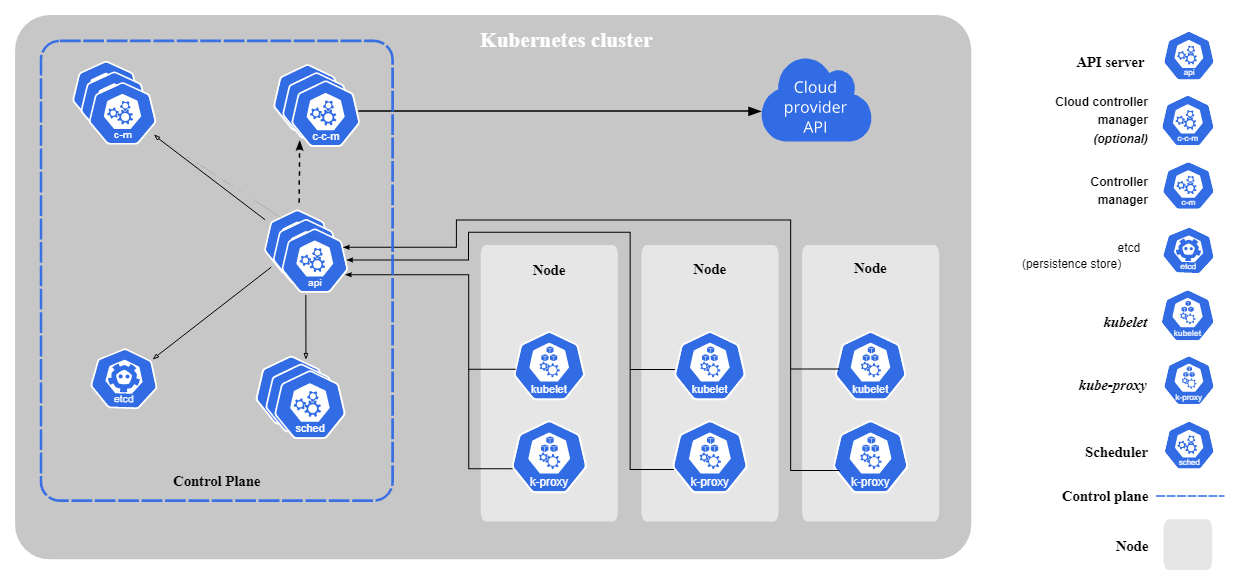
\includegraphics[width=0.7\linewidth]{Pics/kube-architecture}
					\caption{Kiến trúc của Kubernetes}
					\label{fig:kube-architecture}
				\end{figure}
			
				Các thành phần của cụm Kubernetes:\\
				
				\begin{itemize}				
					\item Control Plane: Là trung tâm điều khiển các cụm và làm các cụm kubernetes hoạt động. Đây là nơi quản lý, lên kế hoạch, lập lịch và theo dõi các pod, các node.
					\item Worker Node: Là một máy ảo hoặc máy vật lý chạy Kubernetes. Đây là nơi container thực sự được triển khai để chạy các ứng dụng.
				\end{itemize}
			
				{\hspace{0.3cm}Các thành phần của Control Plane:\\}
				
				\begin{itemize}				
					\item Kubernetes API server: Nơi mà các quản trị viên và các thành phần khác của Control Plane giao tiếp với nhau.
					\item Scheduler: lập lịch cho các ứng dụng của bạn (chỉ định các workload ví dụ như pods được triển khai ở worker node nào)
					\item  Controller Manager: thực hiện các chức năng cấp cụm, chẳng hạn như nhân bản các thành phần, theo dõi các node, xử lý các node lỗi,...
					\item etcd: một kho dữ liệu phân tán đáng tin cậy lưu trữ cấu hình của các node dưới dạng key value.
				\end{itemize}
			
				{\hspace{0.3cm}Các thành phần của Worker Node:\\}
				
				\begin{itemize}				
					\item kubelet: dùng để giao tiếp với API server và quản lý các container nằm trong node.
					\item kube-proxy: là một proxy chạy trên các node trong  Kubernetes. kube-proxy duy trì các quy tắc mạng trên các nút. Các quy tắc mạng này cho phép các Pods trong cùng một node hoặc khác node có thể giao tiếp với nhau.
					\item container-runtime: có thể là Docker, rkt, containerd hoặc một loại container-runtime khác.
				\end{itemize}
			
			\subsection{Tổng quan về Pod}
				{\hspace{0.6cm}Pod là đơn vị thực thi cơ bản của 1 ứng dụng Kubernetes, là đơn vị nhỏ nhất và đơn giản nhất trong mô hình object của Kubernetes. Một Pod đại diện cho các process (tiến trình) chạy trên cluster.\\}
				
				Pod đóng gói một container của ứng dụng (hoặc trong một số trường hợp là nhiều container), tài nguyên lưu trữ, một định danh network duy nhất (địa chỉ IP) cũng như các tùy chọn chi phối cách thức các container sẽ chạy. Một Pod đại diện cho một đơn vị triển khai: một instance (phiên bản) của một ứng dụng trong Kubernetes, có thể chứa một container hoặc vài container được liên kết chặt chẽ và chia sẻ tài nguyên.\\
				
				Docker là container runtime phổ biến nhất được sử dụng cho Pod trong Kubernetes, tuy nhiên Pods cũng hỗ trợ các container runtime khác.\\
				
				Pod trong Kubernetes cluster có thể được sử dụng theo hai cách chính:\\
				\begin{itemize}				
					\item Pods chạy một container duy nhất. Mô hình “một-container-một-Pod” là trường hợp sử dụng phổ biến nhất của Kubernetes; trong trường hợp này, ta có thể nghĩ về một Pod như một trình bao bọc (đóng gói) xung quanh một container và Kubernetes quản lý các Pod thay vì quản lý trực tiếp các container.
					\item Pods chạy nhiều container cần tương tác với nhau. Một Pod có thể đóng gói một ứng dụng chứa nhiều container cùng hoạt động và được liên kết chặt chẽ với nhau cũng như cần chia sẻ tài nguyên (được gọi là co-located container). Các co-located container này có thể tạo thành một đơn vị dịch vụ gắn kết duy nhất nghĩa là 1 container phục vụ các file từ một volume chia sẻ cho public, trong khi đó, một “sidecar” container khác sẽ làm mới (refresh) hoặc cập nhật các file đó. Pod đóng gói các container và tài nguyên lưu trữ này lại với nhau như một thực thể có thể quản lý được.
				\end{itemize}
			\subsection{Vòng đời của Pod}
				{\hspace{0.6cm}Giống như các container, Pod được coi là các thực thể tạm bợ, không bền vững(thay vì lâu bền). Các Pod được tạo, gán một ID (UID) duy nhất và được lên lịch cho các node mà chúng vẫn duy trì cho đến khi bị hủy bỏ (theo chính sách khởi động lại) hoặc xóa. Nếu một node chết, các Pod được lập lịch cho node đó sẽ được lập lịch để xóa sau một khoảng thời gian chờ.\\}
				
				Pod không tự chữa lành. Nếu một Pod được lên lịch cho một node sau đó không thành công, Pod đó sẽ bị xóa; tương tự như vậy, một Pod sẽ không tồn tại sau khi bị trục xuất do thiếu tài nguyên hoặc bảo trì Node. Kubernetes sử dụng phần trừu tượng cấp cao hơn, được gọi là bộ điều khiển, xử lý công việc quản lý các cá thể Pod tương đối dùng một lần.\\
				
				Một Pod nhất định (như được xác định bởi UID) không bao giờ được "lên lịch" đến một nút khác; thay vào đó, Pod đó có thể được thay thế bằng một Pod mới, gần giống, thậm chí có cùng tên nếu muốn, nhưng với một UID khác.\\
				
				Giai đoạn của Pod là một bản tóm tắt đơn giản về vị trí của Pod trong vòng đời của nó.Các giai đoạn của Pod:
				\begin{itemize}				
					\item Pending: Pod đã được chấp nhận bởi hệ thống kubernetes, nhưng 1 hoặc vài container image chưa được tạo ra. Nó bao gồm thời gian trước khi được lập lịch cũng như thời gian download image trên mạng về (có thể mất một lúc)
					\item Running: Pod đã được đưa vào 1 node và tất cả các container đã được tạo ra. Ít nhất 1 container vẫn đang chạy hoặc đang ở trong quá trình bắt đầu hoặc khởi động lại.
					\item  Succeeded: Tất cả các container trong pod đã kết thúc thành công và sẽ không được khởi động lại nữa.
					\item  Failed: Tất cả các container trong pod đã kết thúc và ít nhất 1 contrainer đã thất bại trong quá trình kết thúc. Có nghĩa là container đã exited (thoát) với trạng thái non-zero hoặc đã bị kết thúc bởi hệ thống.
					\item  Unknown: Vì một số lý do, trạng thái của pod không thể xác định được, thường là do bị lỗi trong việc giao tiếp với host của pod.
				\end{itemize}
			\subsection{Quản lí pod bằng Workload trên Kubernetes}
				{\hspace{0.6cm}Workload là một ứng dụng chạy trên Kubernetes. Cho dù workload là một thành phần đơn lẻ hay nhiều thành phần hoạt động cùng nhau, trên Kubernetes, chúng chạy bên trong một tập hợp các pod. Trong Kubernetes, Pod đại diện cho một tập hợp các container đang chạy trên cụm của bạn.\\}
				
				Các Pod có một vòng đời xác định. Ví dụ: khi một Pod đang chạy trong cụm thì một lỗi nghiêm trọng trên node nơi pod đó đang chạy có nghĩa là tất cả các pod trên node đó đều bị lỗi. Kubernetes coi mức độ thất bại đó là cuối cùng: bạn sẽ cần tạo một Pod mới để khôi phục, ngay cả khi node sau đó trở lại bình thường.\\
				
				Tuy nhiên, để làm cho công việc dễ dàng hơn, chúng ta không cần phải quản lý trực tiếp từng Pod. Thay vào đó, bạn có thể sử dụng các workload để quản lý một nhóm các Pod. Các tài nguyên này định cấu hình bộ điều khiển để đảm bảo số lượng phù hợp của loại Pod phù hợp đang chạy, phù hợp với trạng thái chúng ta đã cấu hình.\\
				
				Kubernetes cung cấp một số workload tích hợp sẵn:
				\begin{itemize}				
					\item Deployment và ReplicaSet (thay thế cho ReplicationController). Deployment rất phù hợp để quản lý workload không trạng thái trên cụm, nơi bất kỳ Pod nào trong Deployment đều có thể hoán đổi cho nhau và có thể được thay thế nếu cần.
					\item StatefulSet là workload API object được dùng để quản lý các ứng dụng stateful (có trạng thái). Nó quản lý việc triển khai và co giãn (scale) các pod và cung cấp sự đảm bảo về thứ tự và tính duy nhất của các pod này.
					\item  Một DeamonSet đảm bảo rằng tất cả hoặc một vài node sẽ chạy 1 bản sao của pod. Khi các node được thêm vào cluster thì pod sẽ được lập lịch vào chúng.
					\item  Job và CronJob xác định các nhiệm vụ chạy đến khi hoàn thành và sau đó dừng lại. Công việc đại diện cho các nhiệm vụ một lần, trong khi CronJobs lặp lại theo lịch trình.
				\end{itemize}
		\section{Một số vấn đề bảo mật kiến trúc Microservices}
			{\hspace{0.6cm}Trong hầu hết các ứng dụng được xây dựng trên cấu trúc monolith, bảo mật được thực thi tập trung và các thành phần riêng lẻ không cần phải lo lắng về việc thực hiện các kiểm tra bảo mật trừ khi có yêu cầu. Kết quả là, mô hình bảo mật của một ứng dụng dựa trên cấu trúc monolith là đơn giản hơn nhiều so với ứng dụng được xây dựng dựa trên cấu trúc microservices. Sau đây là một số vấn đề về bảo mật của kiến trúc Microservices gặp phải.\\}			
			\subsection{Càng nhiều microservices thì nguy cơ bị tấn công càng cao}
				{\hspace{0.6cm}Trong một ứng dụng được xây dựng trên cấu trúc monolith, giao tiếp giữa các thành phần bên trong xảy ra trong một tiến trình duy nhất — ví dụ: trong một ứng dụng Java, trong cùng một Máy ảo Java (JVM). Theo kiến trúc microservices, các thành phần bên trong đó được thiết kế dưới dạng các microservices riêng biệt, độc lập và các tiến trình phải gọi lẫn nhau để trao đổi các thông tin. Ngoài ra, mỗi microservice hiện chấp nhận các request một cách độc lập hoặc có các điểm truy cập riêng. Thay vì một vài điểm truy cập, như trong một ứng dụng xây dựng trên cấu trúc monolith, bây giờ chúng ta có số lượng lớn các điểm truy cập. Khi số lượng truy cập vào hệ thống tăng lên, chúng ta sẽ có nhiều điểm bị tấn công hơn. Vấn đề này là một trong những thách thức cơ bản trong việc xây dựng thiết kế bảo mật cho microservices.\\}
			\subsection{Kiểm tra bảo mật phân tán có thể dẫn đến hiệu suất giảm}
				{\hspace{0.6cm}Không giống như trong một ứng dụng được xây dựng trên cấu trúc monolith, mỗi microservice trong triển khai microservices phải thực hiện kiểm tra an ninh độc lập. Từ quan điểm của một ứng dụng dựa trên cấu trúc monolith, trong đó việc kiểm tra bảo mật được thực hiện một lần và các request được gửi đến thành phần tương ứng, nhưng đối với các microservice chúng ta phải kiểm tra tất các các điểm truy cập của chúng. Ngoài ra, trong khi xác thực các yêu cầu tại mỗi microservice, bạn có thể cần kết nối với dịch vụ mã thông báo bảo mật từ xa (STS). Các kiểm tra bảo mật phân tán, lặp đi lặp lại và kết nối từ xa này có thể làm tăng độ trễ và làm giảm đáng kể hiệu suất của hệ thống.\\}
				
				Một số giải quyết vấn đề này bằng cách đơn giản là tin tưởng vào mạng và tránh kiểm tra bảo mật các microservice. Theo thời gian, mạng tin cậy đã trở thành lỗi thời và đang tiến tới các nguyên tắc mạng không tin cậy. Với nguyên tắc mạng không tin cậy, chúng ta thực hiện bảo mật với từng tài nguyên trong mạng. Mọi thiết kế bảo mật microservices phải có hiệu suất tổng thể có thể chấp nhận được.
			\subsection{Sự phức tạp khi triển khai xác thực khởi động giữa các	microservices}
				{\hspace{0.6cm}Giao tiếp dịch vụ với dịch vụ diễn ra giữa các microservice. Mỗi kênh liên lạc giữa các microservice phải được bảo vệ. Chúng có nhiều tùy chọn, nhưng giả sử rằng chúng ta sử dụng chứng chỉ (certificates).\\}
				
				Giờ đây, mỗi microservice phải được cấp chứng chỉ (và khóa bí mật tương ứng), chứng chỉ này sẽ sử dụng để xác thực chính nó với một microservice khác trong quá trình tương tác giữa dịch vụ với dịch vụ. Microservice của người nhận phải biết cách xác thực chứng chỉ được liên kết với microservice đang gọi. Do đó cần một cách để tin tưởng bootstrap giữa các microservices. Ngoài ra cần có khả năng thu hồi chứng chỉ (trong trường hợp khóa bí mật tương ứng bị xâm phạm) và cấp các chứng chỉ mới (thay đổi chứng chỉ định kỳ để giảm thiểu mọi rủi ro khi vô tình làm mất chìa khóa). Những tác vụ này rất cồng kềnh và trừ khi chúng ta tìm ra cách tự động hóa chúng.\\
			\subsection{Khó theo dõi các request của các microservice}
				{\hspace{0.6cm}Khả năng giám sát là thước đo những gì có thể suy ra về trạng thái bên trong của một hệ thống dựa trên kết quả đầu ra bên ngoài của nó. Nhật ký (logs), chỉ số (metrics) và dấu vết (traces) được coi là ba trụ cột của khả năng giám sát.\\}
				
				Nhật ký có thể là bất kỳ sự kiện nào bạn ghi lại tương ứng với một dịch vụ nhất định.\\
				
				Tổng hợp một tập hợp các nhật ký có thể tạo ra các chỉ số. Theo một cách nào đó, các chỉ số phản ánh trạng thái hệ thống. Ví dụ về mặt bảo mật, các yêu cầu truy cập không hợp lệ trung bình mỗi giờ là một chỉ số.\\
				
				Dấu vết cũng dựa trên nhật ký nhưng cung cấp một góc nhìn khác về hệ thống. Theo dõi giúp bạn theo dõi một yêu cầu từ điểm mà nó đi vào hệ thống đến chỉ nơi nó rời khỏi hệ thống. Quá trình này trở nên khó khăn trong mô hình microservices. Không giống như trong một ứng dụng theo cấu trúc monolith, một yêu cầu triển khai microservices có thể xâm nhập vào hệ thống thông qua một microservice và trải dài trên nhiều microservices trước khi nó rời khỏi hệ thống.			
			\subsection{Tính bất biến của container làm việc xác thực và chính sách kiểm soát truy cập của các dịch vụ khó khăn}
				{\hspace{0.6cm}Máy chủ không thay đổi trạng thái sau khi quay được gọi là máy chủ bất biến. Các mô hình triển khai phổ biến nhất cho microservices là dựa trên container. Mỗi microservice chạy bằng container riêng của nó và tất nhiên, container phải là một máy chủ bất biến. Nói cách khác, sau khi container khởi động, nó sẽ không thay đổi bất kỳ tệp nào trong hệ thống tệp của nó hoặc duy trì bất kỳ trạng thái của nó không thay đổi lúc nó đang chạy.\\}
				
				Tính bất biến có tác động gì đến bảo mật và tại sao khái niệm máy chủ bất biến lại được coi là thách thức bảo mật microservices? Trong kiến trúc bảo mật microservices, mỗi microservice trở thành một điểm cần được bảo mật. Do đó, cần duy trì danh sách các máy khách được phép (có thể là các microservice khác) có thể truy cập vào microservice này và cần một bộ chính sách kiểm soát truy cập. Những danh sách này không tĩnh; chúng ta cần được phép cập nhật các danh sách này. Nhưng với tính chất bất biến của container, chúng ta không thể update hệ thống tệp trong các container của các microservice.
			\subsection{Kiến trúc đa ngôn ngữ đòi hỏi các developer phải có thêm nhiều kiến thức bảo mật hơn}
				{\hspace{0.6cm}Trong triển khai microservices, các dịch vụ nói chuyện với nhau qua mạng. Họ không phụ thuộc vào việc triển khai từng dịch vụ, mà phụ thuộc vào giao diện dịch vụ. Tình huống này cho phép mỗi microservice chọn ngôn ngữ lập trình của riêng mình và nền tảng công nghệ để triển khai. Trong một môi trường, trong đó mỗi đội development triển khai các mircoservice của riêng mình, mỗi nhóm có thể linh hoạt để chọn các stack công nghệ để phù hợp với sản phẩm. Kiến trúc này, cho phép các các thành phần trong hệ thống để chọn công nghệ tốt nhất cho chúng, được gọi là một kiến trúc đa ngôn ngữ.\\}
				
				Một kiến trúc đa ngôn ngữ làm cho vấn đề bảo mật trở nên khó khăn. Bởi vì các đội khác nhau sử dụng các stack công nghệ khác nhau để phát triển, mỗi nhóm phải có các chuyên gia bảo mật riêng. Các chuyên gia này phải chịu trách nhiệm xác định các phương pháp bảo mật tốt nhất và hướng dẫn, nghiên cứu các công cụ bảo mật cho mỗi stack công nghệ để phân tích mã nguồn tĩnh và thử nghiệm động và tích hợp các công cụ đó vào quá trình xây dựng. Trách nhiệm của một nhóm bảo mật tập trung, nhưng bây giờ chia vào các đội development. Điều này làm cho các đội development không chú tâm vào việc phát triển sản phẩm mà phải lo một phần về bảo mật nữa làm cho chất lượng sản phẩm giảm do phải viết các module bảo mật làm cho mã nguồn bị rối và khó đọc.
				
				
		\section*{Kết luận Chương 1}
	
	\chapter{Tổng quan về Istio}
		\section{Tổng quan về Istio}
			\subsection{Tổng quan về Service Mesh}
			\subsection{Kiến trúc của Istio}
		\subsection{Tổng quan về Envoy Proxy}
		\section{Quản lý mạng giữa các Microservices với Istio}
			\subsection{Tổng quan về Istio Ingress Gateway}
			\subsection{Định tuyến trong Istio}
			\subsection{Giải quyết các vấn đề về mạng trong Microservices}
		\section{Giám sát các Microservices với Istio}
			\subsection{Một số Metrics quan trọng của Istio}
			\subsection{Giám sát các lưu lượng mạng qua Jaeger và Kiali}
		\section{Bảo mật các Microservices bằng Istio}
			\subsection{Xác thực giữa các Microservices với Istio}
			\subsection{Phân quyền cho các Microservices với Istio}
		\section*{Kết luận chương 2}
	\chapter{Triển khai Istio trên Kubernetes}
		\section{Mô hình triển khai}
		\section{Kịch bản triển khai}
		\section{Thực nghiệm}
		\section{Kết luận}
	
\end{document}